\documentclass{beamer}
\usetheme{Madrid}
\usecolortheme{whale}

\usepackage{appendixnumberbeamer}
\usepackage{multimedia}
\usepackage{braket}
\usepackage{array}
\definecolor{mypurple}{RGB}{255,0,255}

\newcommand{\abs}[1]{\left\lvert #1 \right\rvert}
\graphicspath{ {Graphics/}  }
\setbeamerfont{caption}{size=\scriptsize}

\title[Ba-Yb Quantum Computing]{Scalable Quantum Computation with Ion Chains}
\subtitle{Exploring Using Barium Ions to Sympathetically Cool a Ytterbium Ion Quantum Computer}
\author[J. Wright]{John Wright}
\institute[UW] {
	Department of Physics \\
	University of Washington
}
\date[February 2015]{February 5, 2015}

\begin{document}

\begin{frame}[plain]
\titlepage
\end{frame}

\section{MUSIQC}
\begin{frame}{Ion Trapping}
	\centerline{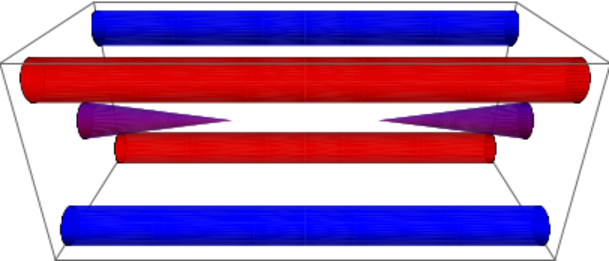
\includegraphics[width=0.7\textwidth]{PaulTrap}}
	\centerline{$V_\mathrm{trap} = \frac{1}{2} m \omega_x^2 x^2 + \frac{1}{2} m \omega_y^2 y^2 + \frac{1}{2} m \omega_z^2 z^2$}
	\vfill
	\centerline{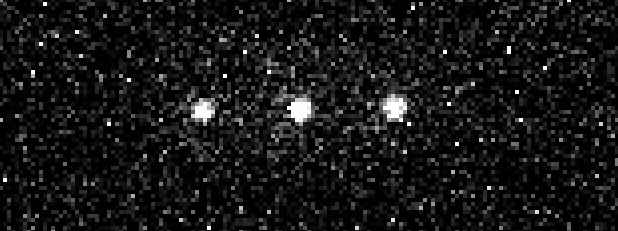
\includegraphics[width=0.5\textwidth]{ThreeIons}}
\end{frame}

\begin{frame}{MUSIQC}
\textbf{Modular Universal Scalable Ion-Trap Quantum Computer Project}
\begin{itemize}
	\item Microfabricated trap designs with many dc control voltages
	\item Separating tasks to different ion species to avoid crosstalk
	\item Entangling ions in separate modular vacuum systems
\end{itemize}
\vfill
\centerline{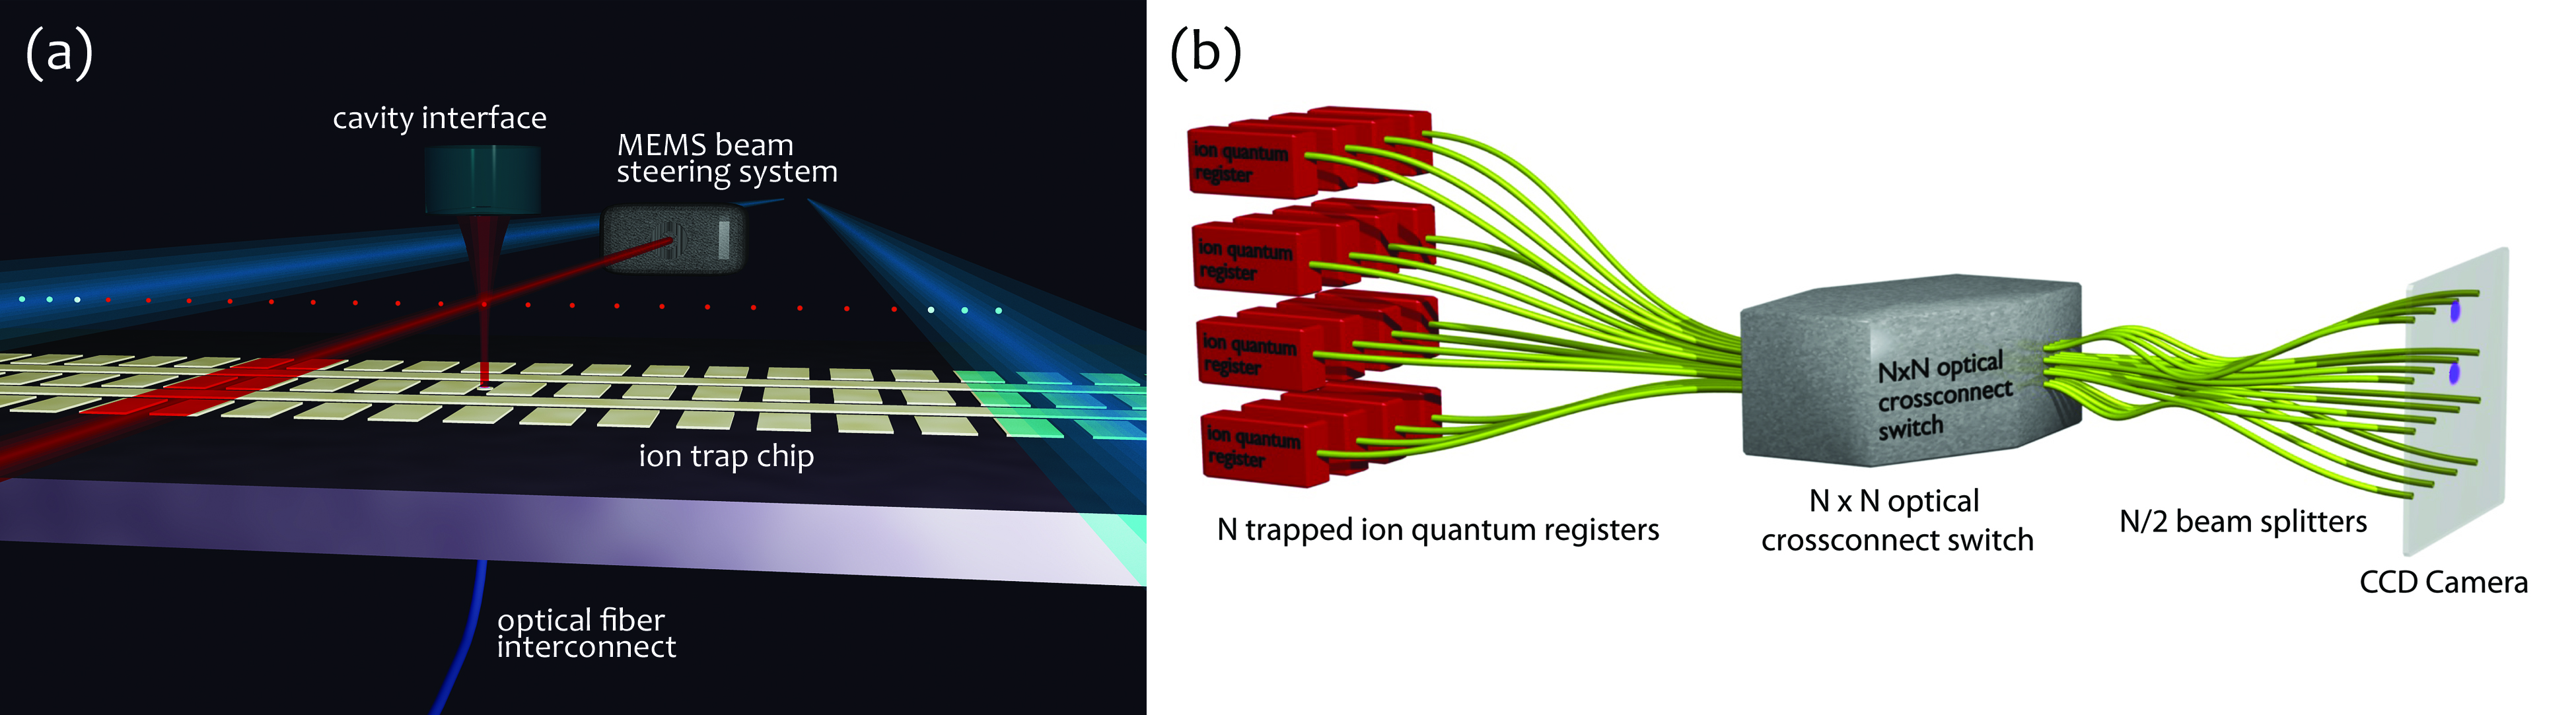
\includegraphics[height=0.38\textheight]{MUSIQC-plan}}
\let\thefootnote\relax\footnote[frame]{C.Monroe, et al, 2012, arXiv:1208.0391}
\end{frame}

\begin{frame}{Surface Ion Traps}
	\centerline{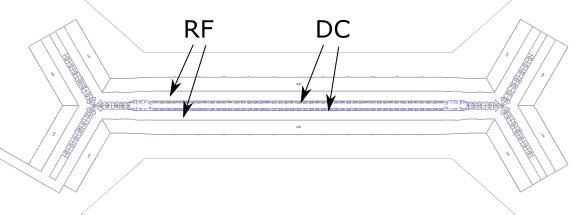
\includegraphics[width=0.9\textwidth]{HOA}}
\end{frame}

\begin{frame}{Boundary Element Method}
	\begin{table}\begin{tabular}{ccc}
		\centering
		& Induced Surface Charges & \\
		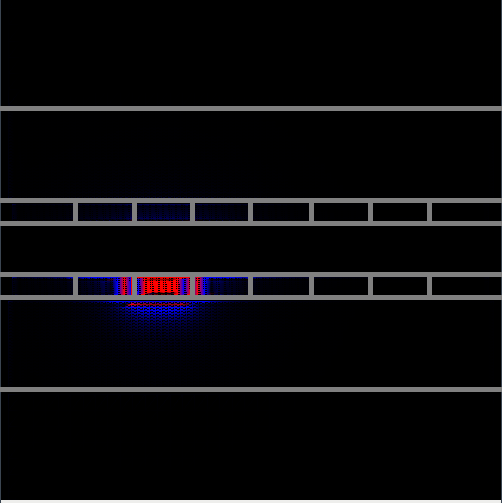
\includegraphics[width=0.3\textwidth]{dc_5} &
		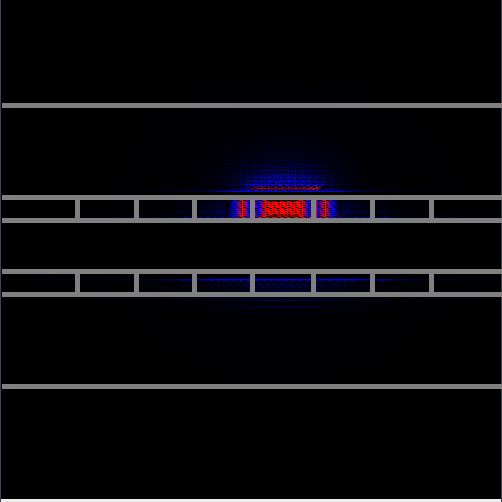
\includegraphics[width=0.3\textwidth]{dc_10} &
		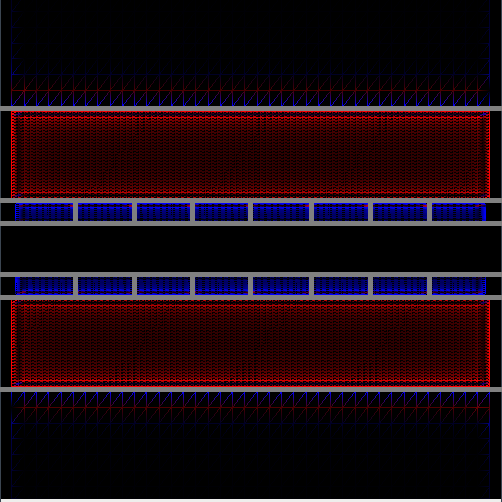
\includegraphics[width=0.3\textwidth]{rf_rails} \\

		
\includegraphics[width=0.3\textwidth]{yz_5} &
		
\includegraphics[width=0.3\textwidth]{yz_10} &
		
\includegraphics[width=0.3\textwidth]{yz_rf} \\
		& Potential in Trap Center &
	\end{tabular}\end{table}
\end{frame}

\begin{frame}{Trapping Solutions}
	\begin{table}\begin{tabular}{cc}
		\centering
		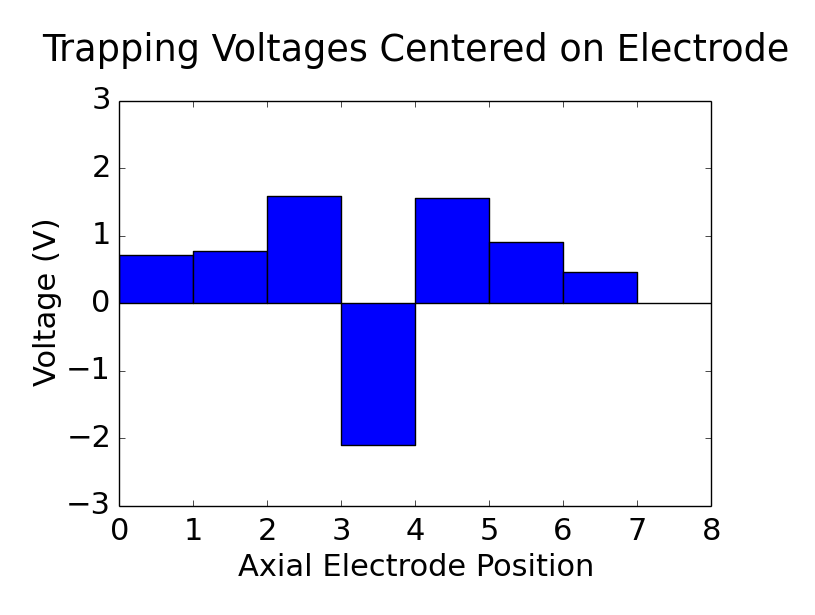
\includegraphics[width=0.4\textwidth]{center_trap} &
		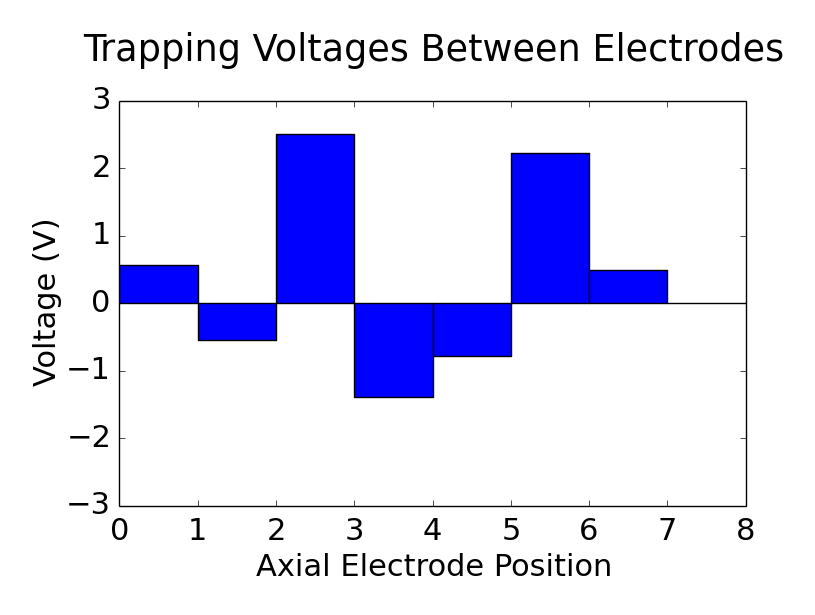
\includegraphics[width=0.4\textwidth]{inbetween_trap}  \\
		
		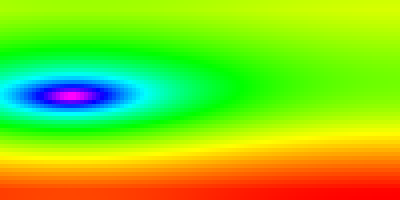
\includegraphics[width=0.4\textwidth]{yz_all_left} &
		
\includegraphics[width=0.4\textwidth]{yz_all}
	\end{tabular}\end{table}
\end{frame}


\begin{frame}{DAC System for DC Control}
	\centering
	\begin{itemize}
		\item 3 AD5372 DAC chips with 32 individually controllable output voltages
		\item Update rates up to 2~MHz via 50~MHz serial interface
		\item Custom FPGA system receives voltages via UDP and buffers updates to saturate DAC interface
	\end{itemize}
	\vfill
	\centerline{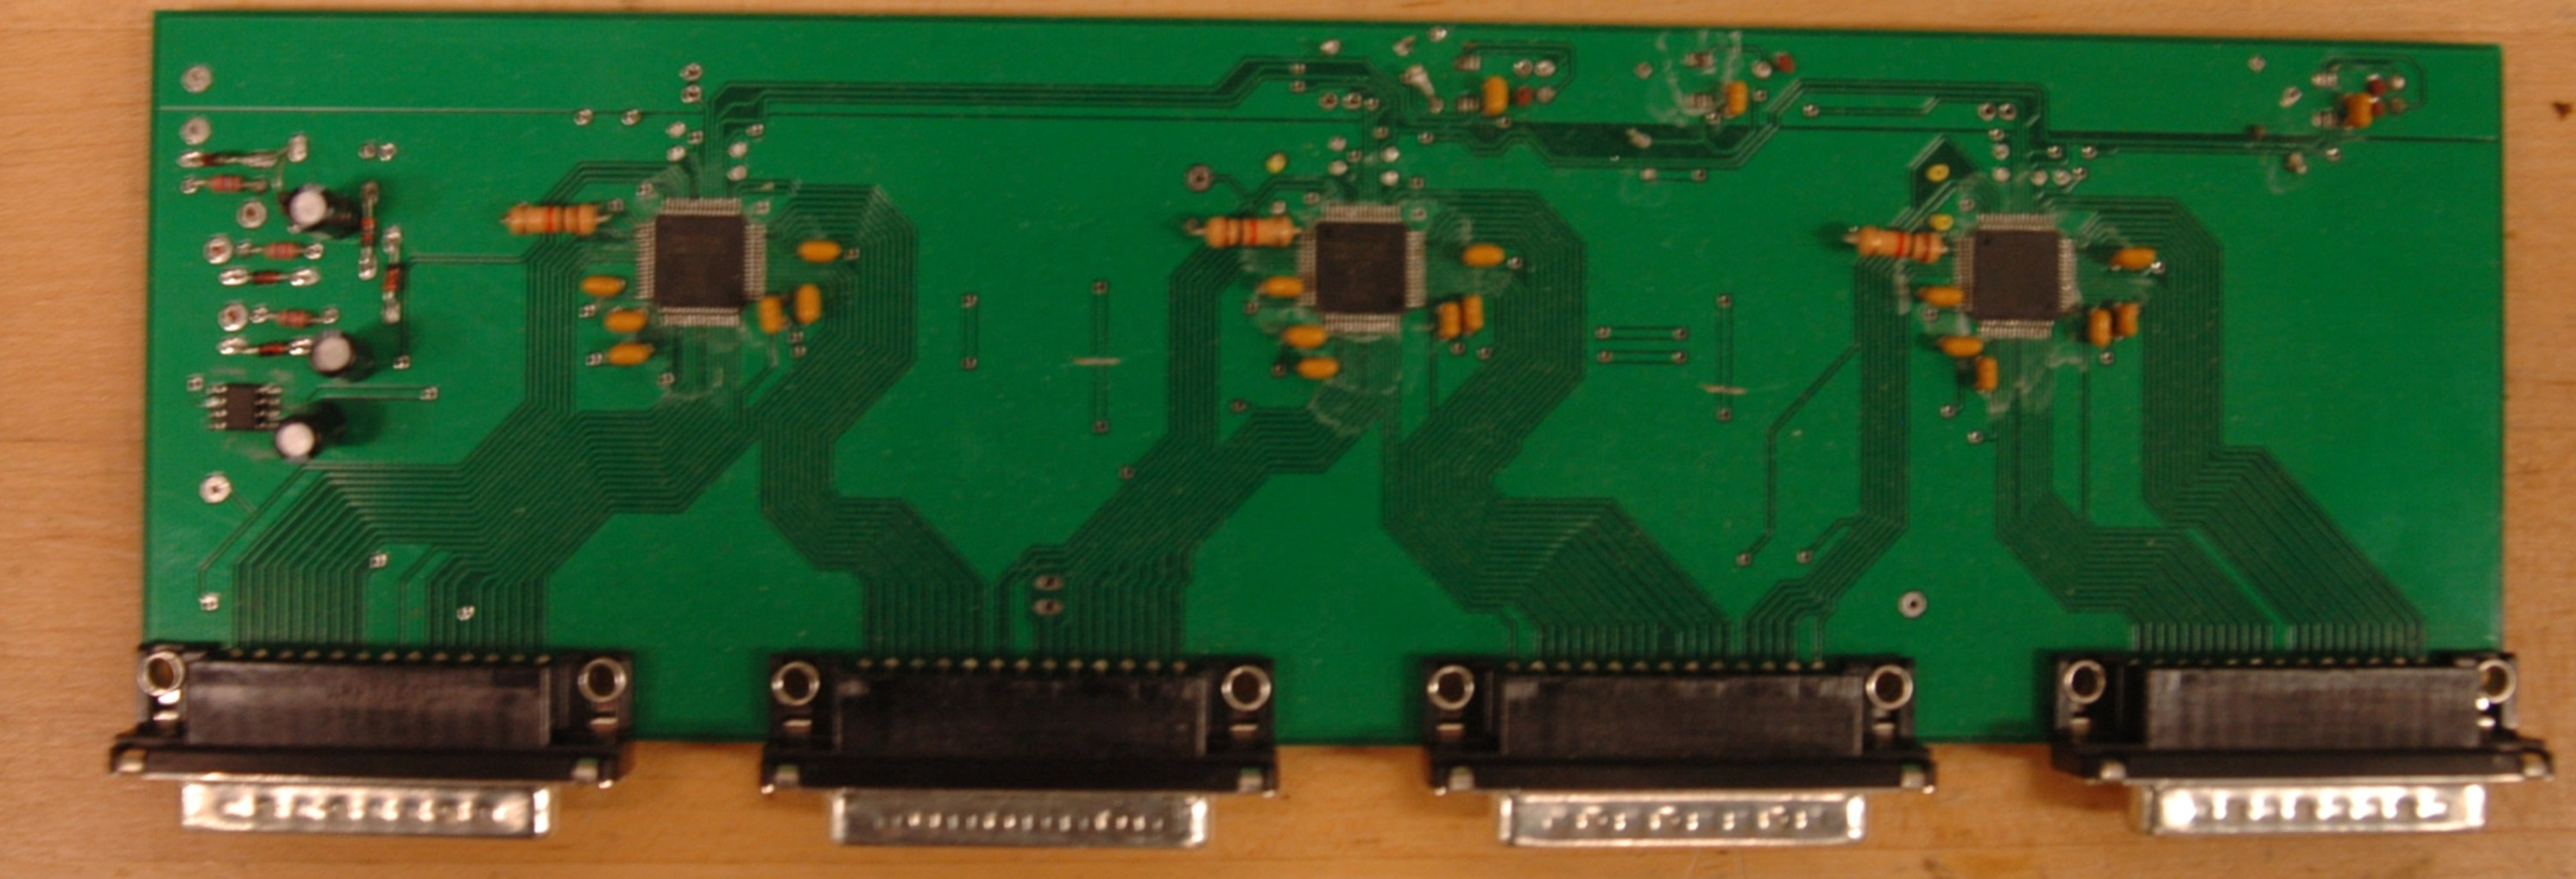
\includegraphics[width=0.8\textwidth]{DAC_board}}
\end{frame}

\begin{frame}{Surface Ion Traps}
	\centerline{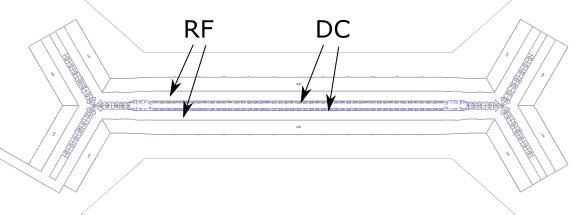
\includegraphics[width=0.9\textwidth]{HOA}}
\end{frame}

\begin{frame}{MUSIQC - Using Multiple Ion Species}
	\centering
	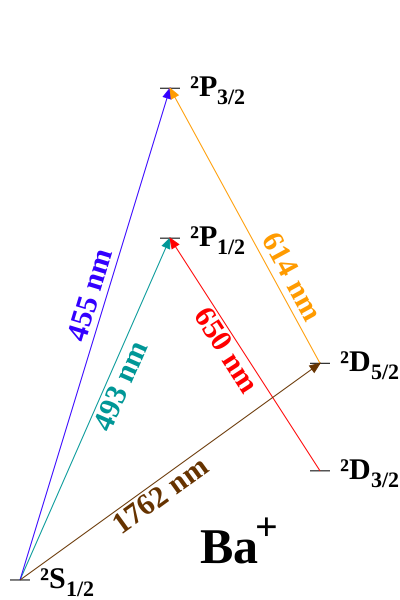
\includegraphics[width=0.4\textwidth]{ionized-Ba}
	\hfill
	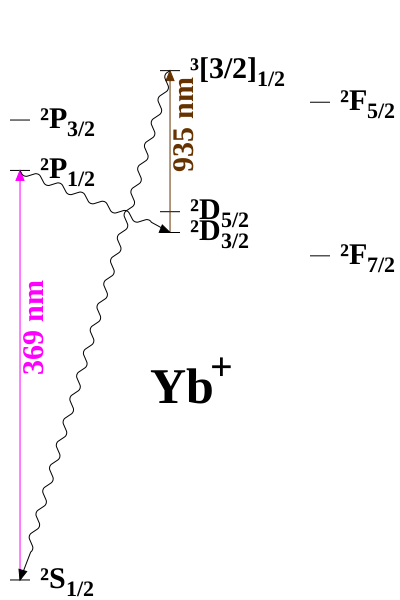
\includegraphics[width=0.4\textwidth]{ionized-Yb}
\end{frame}

\begin{frame}{Mixed Species Chains}
	\centerline{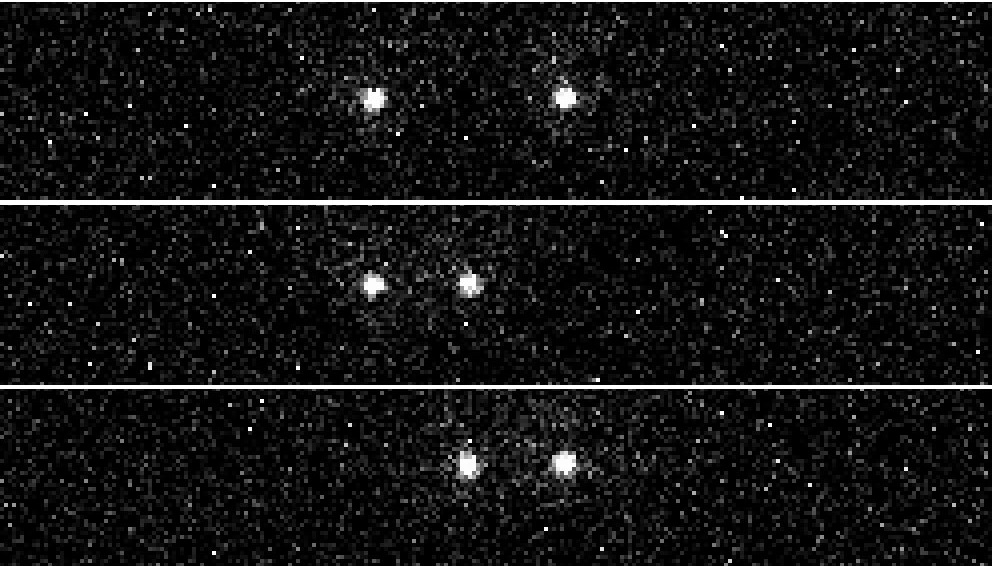
\includegraphics[width=0.5\textwidth]{BaYb}}
	\vfill
	\pause
	\centerline{$V = V_\mathrm{trap} + \frac{1}{2}\sum\limits_{i \ne j}^N \frac{e^2}{4\pi\epsilon_0 \left| \vec{x}_i - \vec{x}_j \right|}$}
	\centerline{$\ddot{\xi}_{a,i} + \sum\limits_{i=1}^{3N} \frac{1}{\sqrt{m_i m_j}} \left( \frac{\partial}{\partial x_i}\frac{\partial}{\partial x_j} V \right) \xi_{a,j} = 0$}
	\centerline{$\xi_{a,i} = e_{a,i} e^{i \omega_a t}$}
\end{frame}

\begin{frame}{Shelving Laser Scans}
	\centering
	\centerline{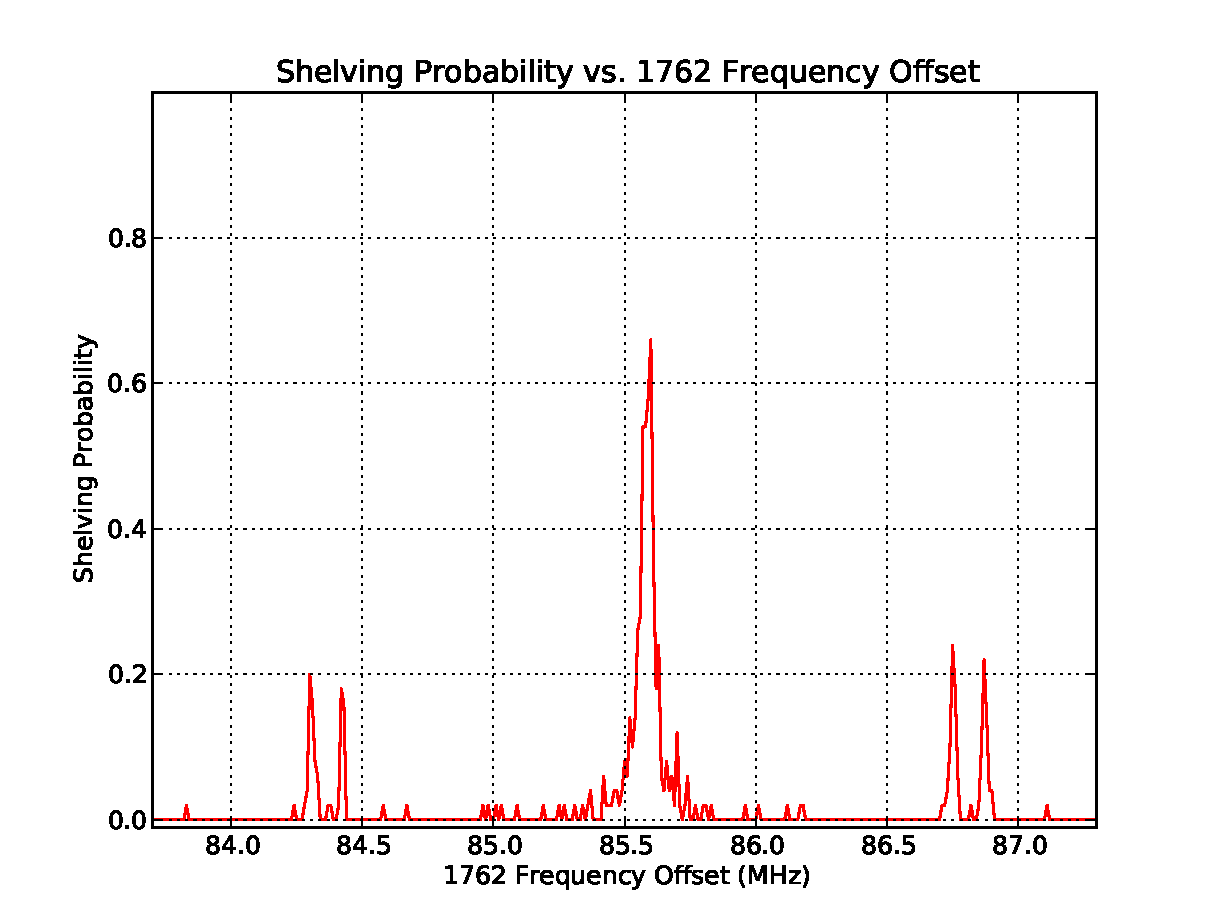
\includegraphics[width=0.75\textwidth]{FullScan}}
	\vfill
	\centerline{${\Large\bra{exc_i}\bra{n_{a} \pm 1}} \vec{u} \cdot \vec{E}(\vec{x}, t) {\Large \ket{n_{a}}\ket{gnd_i}} \propto \sqrt{n_{a}} e_{a,i}$}
\end{frame}

\begin{frame}{Radial Mode Scans}
	\centerline{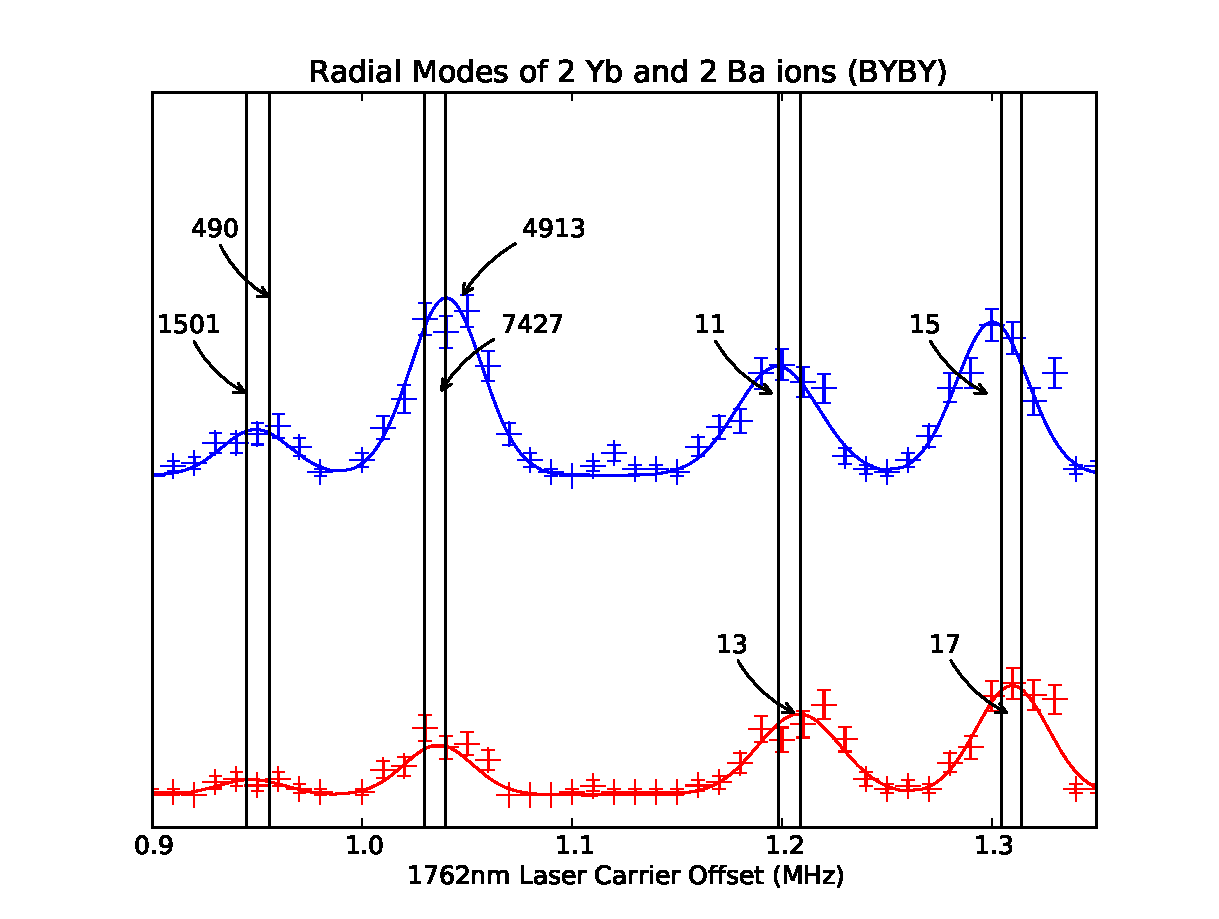
\includegraphics[width=0.9\textwidth]{RadialScanBYBY}}
\end{frame}

\begin{frame}{Radial Mode Scans}
	\centerline{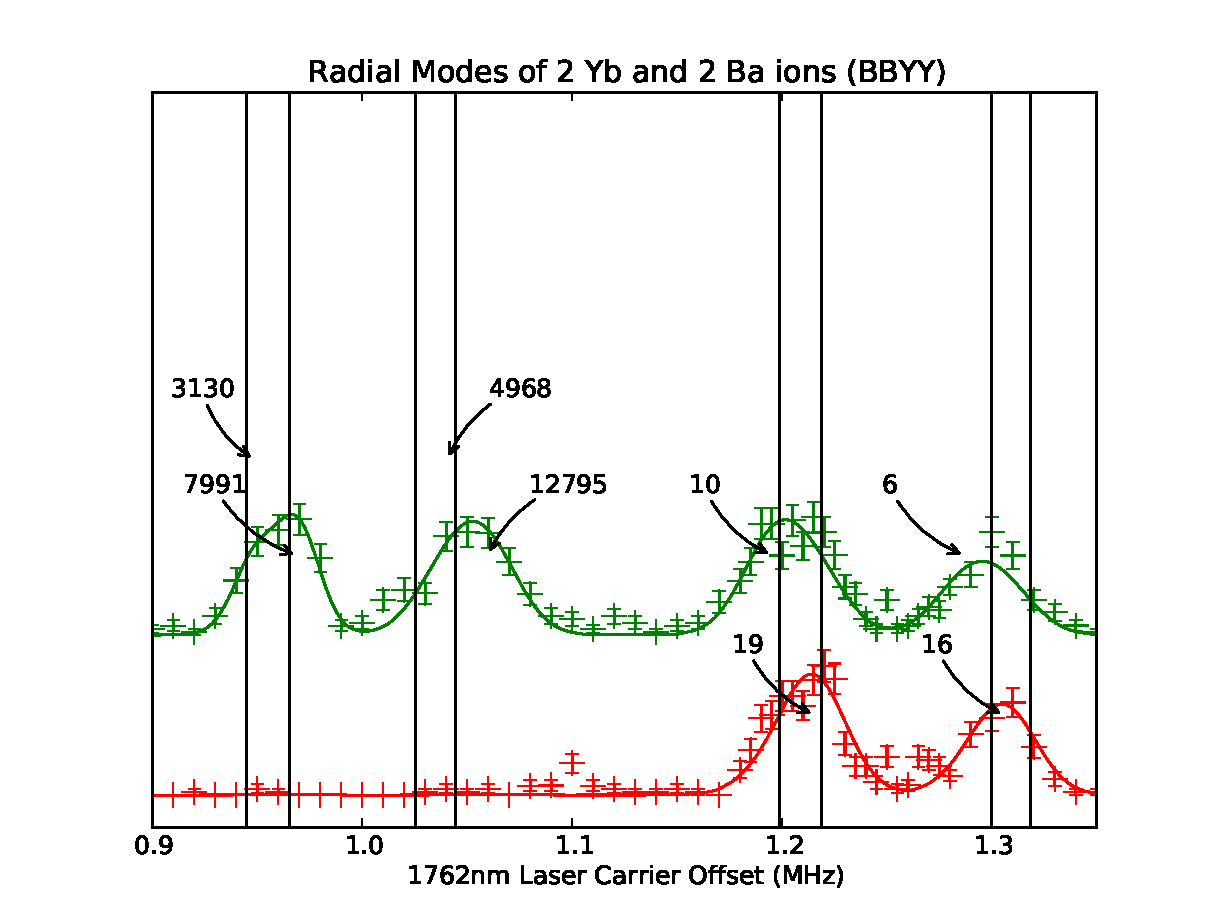
\includegraphics[width=0.9\textwidth]{RadialScanBBYY}}
\end{frame}

\begin{frame}{Radial Mode Scan Results}
	\centerline{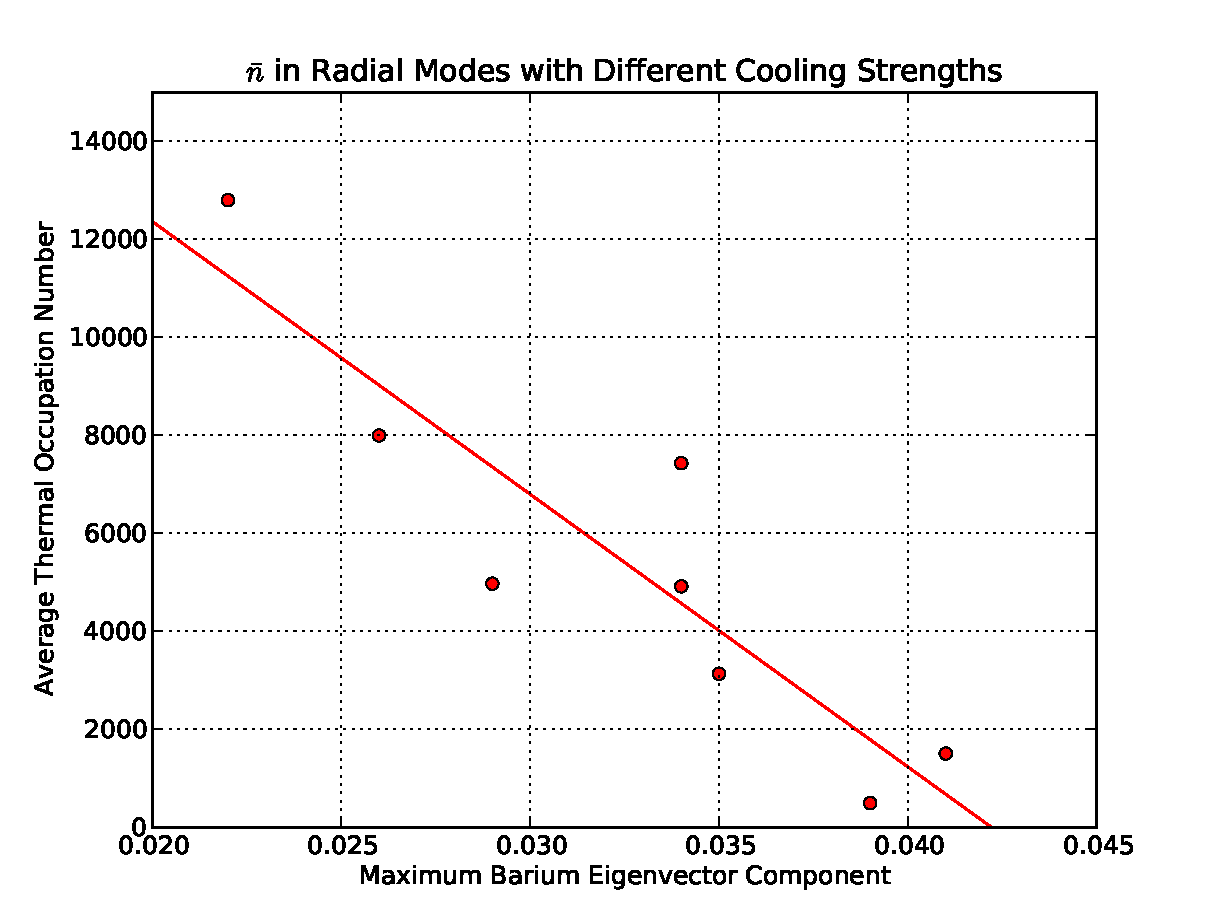
\includegraphics[width=0.9\textwidth]{RadialNBarEigenvectors}}
\end{frame}

\section[]{Conclusions}
\begin{frame}{Conclusions}
\begin{itemize}
	\item MUSQIC program plans to implement a quantum computer with up to 80 qubits which would be capable of outperforming classical computers on specific tasks
	\item Surface ion traps enable us to have separate trapping regions in the same vacuum system and to reorganize ions of different species
	\item Using mixed species chains allows longer quantum operations to be carried out by continuously cooling one ion species
	\item Certain configurations of cooling ions may help preserve the motional states of quantum computing ions longer
\end{itemize}
\end{frame}

\begin{frame}{Thank You}
PI: Boris Blinov
\begin{block}{MUSQIC}
\begin{tabular*}{0.9\textwidth}{ccc}
Tomasz Sakrejda & Richard Graham & Zichao Zhou \\
\end{tabular*}
\end{block}

\begin{block}{Ion Trappers}
\begin{tabular*}{0.9\textwidth}{ccc}
Tom Noel & Carolyn Auchter & Chen-Kuan Chou \\
Matt Hoffman & Spencer Williams & Anupriya Jayakumar \\
Matt Bohman
\end{tabular*}
\end{block}

\begin{columns}
\begin{column}{0.5\textwidth}
	
\includegraphics[width=0.9\textwidth]{musiqc_logo}
\end{column}
\begin{column}{0.5\textwidth}
	
\includegraphics[width=0.9\textwidth]{iarpa}
\end{column}
\end{columns}
\end{frame}

\end{document}
